\documentclass[../../dissertation.tex]{subfiles}
\begin{document}

As was previously seen, the continuous-time quantum walk model is defined by an
evolution operator obtained by solving Schrödinger's equation
\begin{equation}
	U(t) = e^{-iHt}.
\end{equation}
The search problem requires introducing an oracle to the Hamiltonian, that will
mark an arbitrary vertex $m$ 
%meter que pertence a um conjunto de vertices marcados. chamar vertex onde tenho node.
\begin{equation}
	H' = -\gamma L - \sum_{m \in M}\ket{m}\bra{m},
\end{equation}
where $M$ is the set of marked vertices. Since the complete graph is a regular graph, the operator can be rewritten in terms of the adjacency matrix plus the marked elements. Considering the case where only element $\ket{0}$ is marked, one gets
\begin{equation}
	U'(t) = e^{iH't} = e^{i(-\gamma L - \ket{0}\bra{0})t} = e^{i(-\gamma A + \gamma D - \ket{0}\bra{0})t} = e^{-i\gamma(A+\ket{0}\bra{0})t + i\gamma D t}.
\end{equation}
The degree matrix is again $D=dI$, which means it will commute with $A+\ket{0}\bra{0}$ and become a global phase
\begin{equation}
	U'(t) = e^{-i\gamma(A+\ket{0}\bra{0})t}e^{i\gamma D t} = \phi(t)e^{-i\gamma(A+\ket{0}\bra{0})t}.
\end{equation}\par
As was show by \cite{childs2004}, the value of $\gamma$ is crucial for the
success of the search. As $\gamma$ increases, the contribution of the marked
element in the Hamiltonian decreases and, as $\gamma$ approaches $0$, the
contribution of the adjacency matrix decreases. To find the optimum value, the
Hamiltonian can be rewritten by adding multiples of the identity matrix to the
adjacency matrix 
%TODO:\textcolor{red}{H' é uma notação ruim, confunde com derivada e acredito não ser necessário aqui}
\begin{equation}
	H' = -\gamma(A+NI) - \ket{0}\bra{0} = -\gamma N\ket{s}\bra{s} - \ket{0}\bra{0},
\end{equation}
\begin{figure}[h]
	\centering 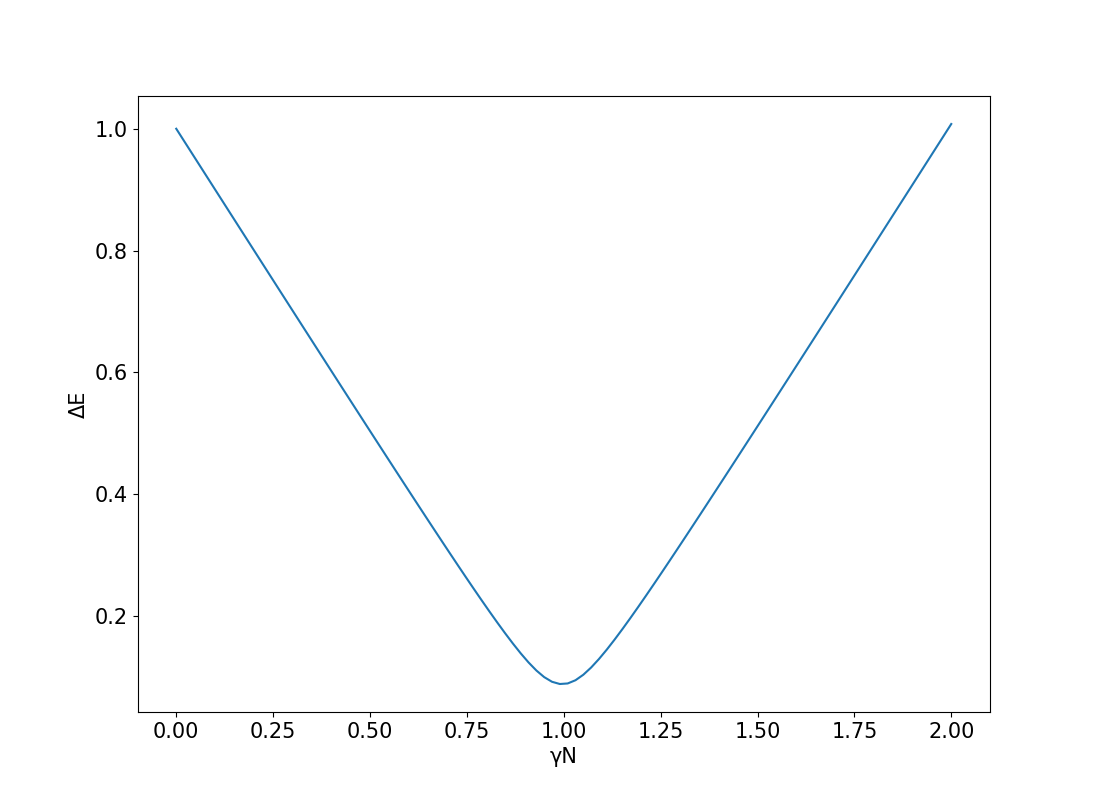
\includegraphics[scale=0.40]{img/ContQuantumWalk/Search/gamma512.png}
	\caption{Value of the difference between the largest eigenvalue and the second largest plotted as a function of $\gamma N$, for $N=512$.}
	\label{fig:gamma512}
\end{figure}
%TODO: Perceber de onde vem o w.
where $\ket{s} = \frac{1}{\sqrt{N}}\sum_i \ket{i}$. Now it is obvious that, for
$\gamma = \frac{1}{N}$, the Hamiltonian becomes $H = -\ket{s}\bra{s} -
\ket{0}\bra{0}$. Its eigenstates are proportional to $\ket{s}\pm\ket{w}$ and
eigenvalues are $-1 - \frac{1}{\sqrt{N}}$ and $-1 + \frac{1}{\sqrt{N}}$,
respectively. This means that the evolution rotates from the state of balanced
superposition to the marked vertex state in time $\frac{\pi}{\Delta E} =
\frac{\pi}{2}\sqrt{N}$ which is, as shown by \cite{farhi2000}, equivalent to
Grover's algorithm.\par

Plotting $\Delta E$ as a function of $\gamma N$, as can be seen in figure
\ref{fig:gamma512}, has a minimum at $\gamma N =1$. The difference between the
largest eigenvalue and second largest, plotted in the y-axis, is the smallest
for a value of $\gamma N = 1 \implies \gamma =\frac{1}{N}$, which will
correspond to the maximum probability for the marked vertex, in optimal steps.\par

Figure \ref{fig:ContSearchProbDist} shows the evolution of the probability of the
marked vertex in time, which is continuous in this model. In contrast with
previous models, the distributions are smooth and reach exactly one, since the
walk is allowed to evolve for exactly the ideal time steps.
%figura da caminhada com passos ideais
\begin{figure}[!t]
	\centering 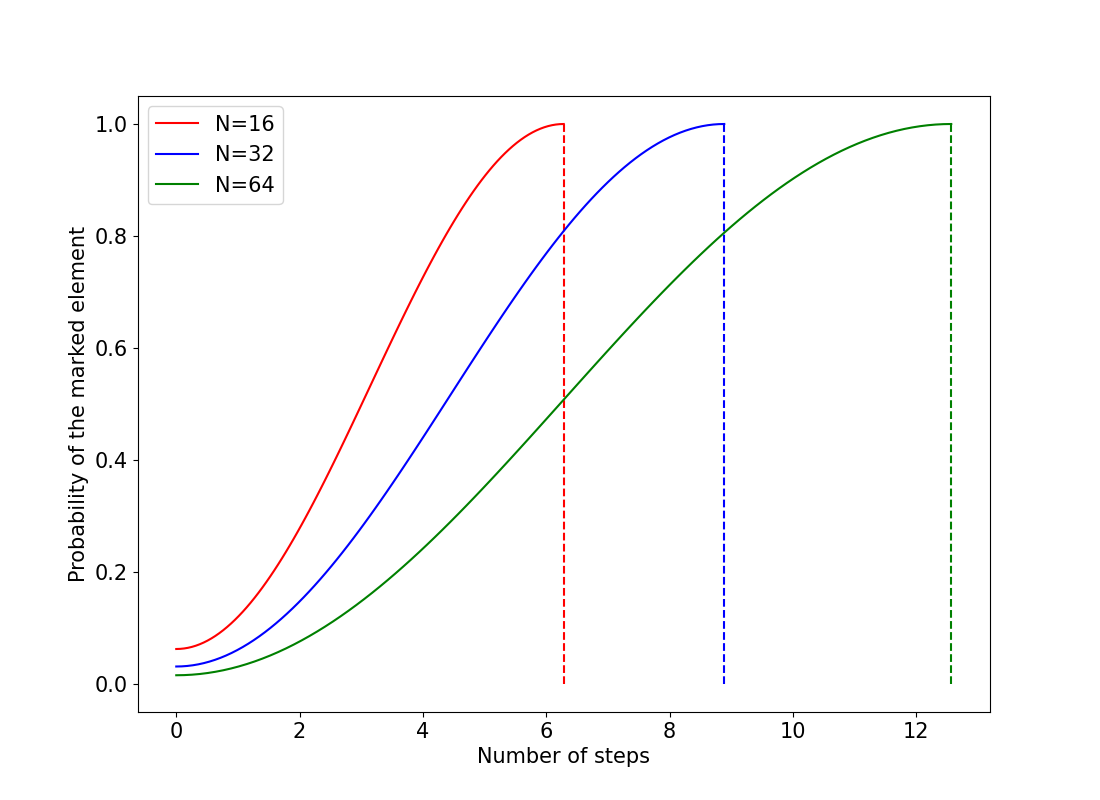
\includegraphics[scale=0.40]{img/ContQuantumWalk/Search/163264.png}
	\caption{Probability of one marked element in the continuous quantum walk search, as a function of the number of steps, for complete graphs of size $N=16$, $32$ and $64$.}\label{fig:ContSearchProbDist}
\end{figure}\par

%TODO: Melhorar este fechamento.
Again, this walk will require only as many qubits as needed to represent the
space of the walker. Similarly to the staggered case, this model allows an
adjustment to the $\gamma$ parameter, that will affect the number of ideal
steps. It also allows the choice of structure over which to perform the
search, making it more general than the Grover algorithm as well. Another
interesting property is that, because time is treated as a continuous variable,
the circuit associated will not scale in time. For the case without
search, the circuit will be relatively small and somewhat resistant to noise.
When considering the search problem, however, the introduction of the oracle
and the dependency of the Suzuki-Trotter expansion will render the circuit less
than ideal for NISQ implementation, as will be seen in the next chapter.

\end{document}
